%!TEX root = ../report.tex

\begin{document}
    \chapter{附加功能}

    How you are planning to test/compare/evaluate your research.
    Criteria used.
	
	\section{键鼠交互的相机旋转移动}
	\begin{lstlisting}
		hello world!
	\end{lstlisting}
	\subsection{平移旋转变换}
	\begin{spacing}{2.5}
	其实,所谓相机的旋转移动可以看成相机固定不动,而物体在进行逆变换,例如,相机左移一个单位其实就是物体向右移动一个单位。因此要相机的旋转移动,只要实现物体对应的旋转移动即可。所用到的变换矩阵如下:
	\begin{enumerate}
		\item 平移变换矩阵
		\begin{equation}
		\begin{pmatrix}
			1 &  0&  0&0 \\ 
 			0&  1&  0& 0\\ 
 			0& 0 & 1 &0 \\ 
 			T_{x}&  T_{y}&  T_{z}& 1
		\end{pmatrix}
		\label{transfer_1}
		\end{equation}
		\item 	绕X轴旋转变换矩阵
		\begin{equation}
		\begin{pmatrix}
			 1&  0&  0 &0 \\ 
 			0&  cos\theta &  sin\theta& 0\\ 
 			 0& -sin\theta & cos\theta &0 \\ 
 			0&  0&  0& 1
		\end{pmatrix}
		\label{yrotate}
		\end{equation}
		\item 绕Y轴旋转变换矩阵
		\begin{equation}
		\begin{pmatrix}
			cos\theta &  0&  -sin\theta &0 \\ 
 			0&  1&  0& 0\\ 
 			sin\theta & 0 & cos\theta &0 \\ 
 			0&  0&  0& 1
		\end{pmatrix}
		\label{xrotate}	
		\end{equation}
	
		\item 绕Z轴旋转变换矩阵
		\begin{equation}
		\begin{pmatrix}
			cos\theta &  sin\theta &  0 &0 \\ 
 			-sin\theta &  cos\theta &  0& 0\\ 
 			0 & 0 & 1 &0 \\ 
 			0&  0&  0& 1
		\end{pmatrix}
		\label{zrotate}
		\end{equation}
		\item 缩放变换矩阵
		\begin{equation}
		\begin{pmatrix}
			S_{x}& 0 &  0 &0 \\ 
 			0 &  S_{y} &  0& 0\\ 
 			0 & 0 & S_{z} &0 \\ 
 			0&  0&  0& 1
		\end{pmatrix}
		\label{zrotate}
		\end{equation}
	\end{enumerate}
	\end{spacing}

    \section{区域填充}

    \section{纹理贴图}
    
    \section{光照}
    \begin{spacing}{2.5}
    \subsection{冯氏光照模型}
    现实世界的光照是很复杂的,物体的材质和光照的特性都会影响最终的渲染效果,在有限的计算能力下,我们很难模拟完全真实的光照条件。因此,图形学的渲染更倾向于使用一种简化的模型对现实情况进行近似。\\
    本次我们参考了OpenGL的处理方式,采用冯氏光照模型(Phong Lighting Model)进行光照模拟。冯氏光照模型的主要结构由3个分量组成:环境(Ambient)、漫反射(Diffuse)和镜面(Specular)光照。下图展示了这些光照分量的影响:\\
    \begin{figure}[H]
    	\centering
		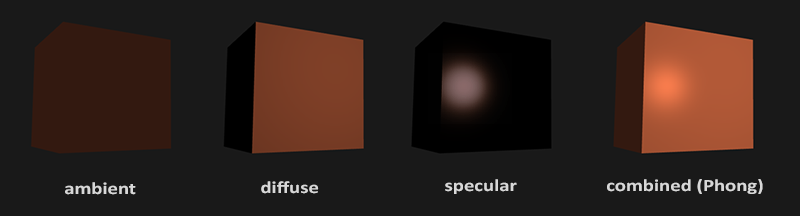
\includegraphics[width=1.0\textwidth]{images/phong_model.png}
		\caption{冯氏光照模型分量}
		\label{phong_model}
    \end{figure}
    
    \begin{itemize}
    	\item 环境光照(Ambient Lighting):即使在黑暗的情况下,世界上通常也仍然有一些光亮(月亮、远处的光),所以物体几乎永远不会是完全黑暗的。为了模拟这个,我们会使用一个环境光照常量,它永远会给物体一些颜色。
    	\item 漫反射光照(Diffuse Lighting):模拟光源对物体的方向性影响(Directional Impact)。它是冯氏光照模型中视觉上最显著的分量。物体的某一部分越是正对着光源,它就会越亮。
    	\item 镜面光照(Specular Lighting):模拟有光泽物体上面出现的亮点。镜面光照的颜色相比于物体的颜色会更倾向于光的颜色。
    \end{itemize}
    
    将上述三个分量全部叠加后即可得到最终的渲染颜色。
    
    \subsection{环境光照}
    
    在现实环境中,光源可能有很多个,并可能通过多个物体进行反射从而简介对其他物体产生影响。考虑到这种情况的算法叫全局光照(Global Illumination)算法,但是这种算法开销极高,且运算较为复杂。\\
    在冯氏光照中采用了最简单的方法模拟环境光照,即用常量因子乘以环境颜色获得一个近似结果,它在代码中的体现如下:
   
   
	\begin{lstlisting}[language={[ANSI]C},numbers=left,numberstyle=\tiny,%frame=shadowbox,
   rulesepcolor=\color{red!20!green!20!blue!20},
   keywordstyle=\color{blue!70!black},
   commentstyle=\color{blue!90!},
   basicstyle=\ttfamily]
	Color PhongShader::getAmbient(const VertexOut &frag) const {
    Color ambient = _ambient.color * _ambient.factor;
    return ambient;
	}
	\end{lstlisting}
	
	\subsection{漫反射光照}
	
	比起环境光照,漫反射光照分量最能产生显著的视觉影响。它的思想是,同光线角度最接近的片段可以获得最高的亮度:
	
	\begin{figure}[H]
    	\centering
		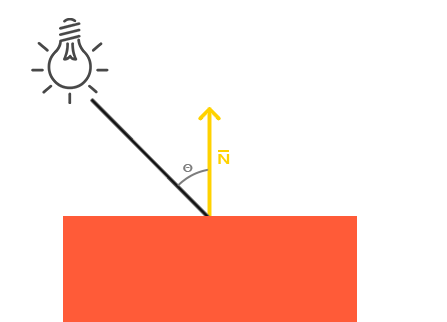
\includegraphics[width=1.0\textwidth]{images/diffuse_light.png}
		\caption{漫反射分量示意图}
		\label{diffuse_light}
    \end{figure}
	
	如图,其中$\overline N$代表其中一个片元的法向量,它与光照方向产生了角度$\theta$;对光线入射向量和法向量分别标准化,之后取两者的点积可以得到$cos\theta$,将该值与光线颜色相乘,取一个比例系数之后得到结果,该值的大小反映了夹角大小的同时也指代了光线的明暗。\\
	值得注意的是,有时候这个点积会得到负值,但这意味着光线与某个法向量成钝角,也就是在片元的“另一边”,此时在实现时只需要将它取为0即可,下面是漫反射分量在代码中的体现:
	
	\begin{lstlisting}[language={[ANSI]C},numbers=left,numberstyle=\tiny,%frame=shadowbox,
   rulesepcolor=\color{red!20!green!20!blue!20},
   keywordstyle=\color{blue!70!black},
   commentstyle=\color{blue!90!},
   basicstyle=\ttfamily]
	double cosTheta = ray.dot(normal);
    double diff = max(cosTheta , (double)0.0f);
    Color diffuse = _light.color* _light.factor * diff * _material.diffuseFactor;
    return diffuse;
	\end{lstlisting}
	
	\subsection{镜面光照}
	
	镜面光照将观察者的观察向量也融入到了渲染之中。假设物体是一面镜子,那么入射的光将被完全反射,此时就必须考虑该反射光和观察者视角对于物体亮度的影响。
	
    \begin{figure}[H]
    	\centering
		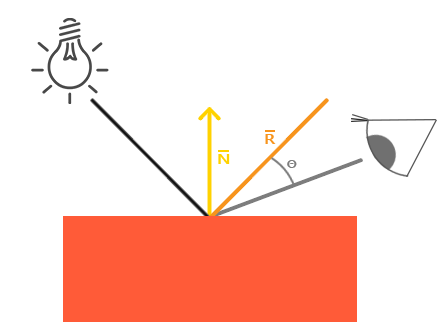
\includegraphics[width=1.0\textwidth]{images/specular_light.png}
		\caption{镜面分量示意图}
		\label{specular_light}
    \end{figure}
    
    如图,我们通过反射法向量周围光的方向来计算反射向量。然后我们计算反射向量和视线方向的角度差,如果夹角越小,那么镜面光的影响就会越大。它的作用效果就是,当我们去看光被物体所反射的那个方向的时候,我们会看到一个高光,它的代码实现如下:
    \begin{lstlisting}[language={[ANSI]C},numbers=left,numberstyle=\tiny,%frame=shadowbox,
   rulesepcolor=\color{red!20!green!20!blue!20},
   keywordstyle=\color{blue!70!black},
   commentstyle=\color{blue!90!},
   basicstyle=\ttfamily]
   Vec3 center = (ray + viewDir).getNormalize();
	 auto spec = pow(max(center.dot(normal), 0.0), _material.shininess);
    Color specular = _light.color * _light.factor * spec * _material.specularFactor;
    return specular;
	\end{lstlisting}
    
    在实现时,计算反射光的法向量比较麻烦,为此,先将入射光单位向量和观察方向单位向量相加求出两者的角平分线,之后再计算角平分线与法向量的夹角,这个计算的合理性如下:
   		\begin{equation}
   			\frac{2\alpha+\theta}{2} - \alpha = \frac{\theta}{2}
   		\end{equation}
    其中,$\alpha$是入射角,$\theta$是待求夹角。\\
    在下一行,将求得的值取了一个次幂,所取的指数叫做反光度(Shininess),一个物体的反光度越高,反射光的能力越强,散射得越少,高光点就会越小。下面的图片反映了不同反光度对渲染效果的影响:
    
    \begin{figure}[H]
    	\centering
		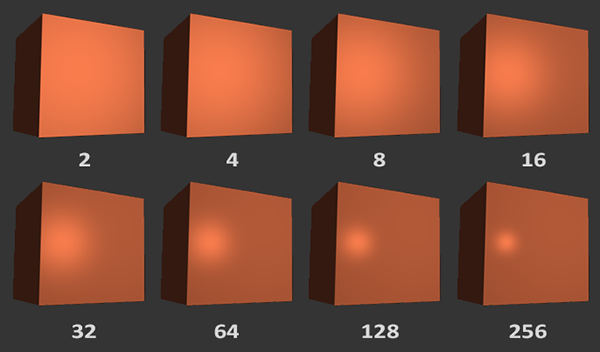
\includegraphics[width=1.0\textwidth]{images/shininess.png}
		\caption{不同反光度的视觉效果}
		\label{shininess}
    \end{figure}
    
    最后,将上述三个分量参数简单相加后乘以物体本身的颜色,即输出冯氏光照的结果。
    	
    \end{spacing}
  

    \section{三维模型}
    
    \section{天空盒子}
    
    
    
\end{document}
